\documentclass[]{article}
\usepackage{lmodern}
\usepackage{amssymb,amsmath}
\usepackage{ifxetex,ifluatex}
\usepackage{fixltx2e} % provides \textsubscript
\ifnum 0\ifxetex 1\fi\ifluatex 1\fi=0 % if pdftex
  \usepackage[T1]{fontenc}
  \usepackage[utf8]{inputenc}
\else % if luatex or xelatex
  \ifxetex
    \usepackage{mathspec}
  \else
    \usepackage{fontspec}
  \fi
  \defaultfontfeatures{Ligatures=TeX,Scale=MatchLowercase}
\fi
% use upquote if available, for straight quotes in verbatim environments
\IfFileExists{upquote.sty}{\usepackage{upquote}}{}
% use microtype if available
\IfFileExists{microtype.sty}{%
\usepackage{microtype}
\UseMicrotypeSet[protrusion]{basicmath} % disable protrusion for tt fonts
}{}
\usepackage[margin=1in]{geometry}
\usepackage{hyperref}
\hypersetup{unicode=true,
            pdftitle={Mapping and Markdown Tutorial},
            pdfauthor={Nicholas Nagle},
            pdfborder={0 0 0},
            breaklinks=true}
\urlstyle{same}  % don't use monospace font for urls
\usepackage{color}
\usepackage{fancyvrb}
\newcommand{\VerbBar}{|}
\newcommand{\VERB}{\Verb[commandchars=\\\{\}]}
\DefineVerbatimEnvironment{Highlighting}{Verbatim}{commandchars=\\\{\}}
% Add ',fontsize=\small' for more characters per line
\usepackage{framed}
\definecolor{shadecolor}{RGB}{248,248,248}
\newenvironment{Shaded}{\begin{snugshade}}{\end{snugshade}}
\newcommand{\AlertTok}[1]{\textcolor[rgb]{0.94,0.16,0.16}{#1}}
\newcommand{\AnnotationTok}[1]{\textcolor[rgb]{0.56,0.35,0.01}{\textbf{\textit{#1}}}}
\newcommand{\AttributeTok}[1]{\textcolor[rgb]{0.77,0.63,0.00}{#1}}
\newcommand{\BaseNTok}[1]{\textcolor[rgb]{0.00,0.00,0.81}{#1}}
\newcommand{\BuiltInTok}[1]{#1}
\newcommand{\CharTok}[1]{\textcolor[rgb]{0.31,0.60,0.02}{#1}}
\newcommand{\CommentTok}[1]{\textcolor[rgb]{0.56,0.35,0.01}{\textit{#1}}}
\newcommand{\CommentVarTok}[1]{\textcolor[rgb]{0.56,0.35,0.01}{\textbf{\textit{#1}}}}
\newcommand{\ConstantTok}[1]{\textcolor[rgb]{0.00,0.00,0.00}{#1}}
\newcommand{\ControlFlowTok}[1]{\textcolor[rgb]{0.13,0.29,0.53}{\textbf{#1}}}
\newcommand{\DataTypeTok}[1]{\textcolor[rgb]{0.13,0.29,0.53}{#1}}
\newcommand{\DecValTok}[1]{\textcolor[rgb]{0.00,0.00,0.81}{#1}}
\newcommand{\DocumentationTok}[1]{\textcolor[rgb]{0.56,0.35,0.01}{\textbf{\textit{#1}}}}
\newcommand{\ErrorTok}[1]{\textcolor[rgb]{0.64,0.00,0.00}{\textbf{#1}}}
\newcommand{\ExtensionTok}[1]{#1}
\newcommand{\FloatTok}[1]{\textcolor[rgb]{0.00,0.00,0.81}{#1}}
\newcommand{\FunctionTok}[1]{\textcolor[rgb]{0.00,0.00,0.00}{#1}}
\newcommand{\ImportTok}[1]{#1}
\newcommand{\InformationTok}[1]{\textcolor[rgb]{0.56,0.35,0.01}{\textbf{\textit{#1}}}}
\newcommand{\KeywordTok}[1]{\textcolor[rgb]{0.13,0.29,0.53}{\textbf{#1}}}
\newcommand{\NormalTok}[1]{#1}
\newcommand{\OperatorTok}[1]{\textcolor[rgb]{0.81,0.36,0.00}{\textbf{#1}}}
\newcommand{\OtherTok}[1]{\textcolor[rgb]{0.56,0.35,0.01}{#1}}
\newcommand{\PreprocessorTok}[1]{\textcolor[rgb]{0.56,0.35,0.01}{\textit{#1}}}
\newcommand{\RegionMarkerTok}[1]{#1}
\newcommand{\SpecialCharTok}[1]{\textcolor[rgb]{0.00,0.00,0.00}{#1}}
\newcommand{\SpecialStringTok}[1]{\textcolor[rgb]{0.31,0.60,0.02}{#1}}
\newcommand{\StringTok}[1]{\textcolor[rgb]{0.31,0.60,0.02}{#1}}
\newcommand{\VariableTok}[1]{\textcolor[rgb]{0.00,0.00,0.00}{#1}}
\newcommand{\VerbatimStringTok}[1]{\textcolor[rgb]{0.31,0.60,0.02}{#1}}
\newcommand{\WarningTok}[1]{\textcolor[rgb]{0.56,0.35,0.01}{\textbf{\textit{#1}}}}
\usepackage{graphicx,grffile}
\makeatletter
\def\maxwidth{\ifdim\Gin@nat@width>\linewidth\linewidth\else\Gin@nat@width\fi}
\def\maxheight{\ifdim\Gin@nat@height>\textheight\textheight\else\Gin@nat@height\fi}
\makeatother
% Scale images if necessary, so that they will not overflow the page
% margins by default, and it is still possible to overwrite the defaults
% using explicit options in \includegraphics[width, height, ...]{}
\setkeys{Gin}{width=\maxwidth,height=\maxheight,keepaspectratio}
\IfFileExists{parskip.sty}{%
\usepackage{parskip}
}{% else
\setlength{\parindent}{0pt}
\setlength{\parskip}{6pt plus 2pt minus 1pt}
}
\setlength{\emergencystretch}{3em}  % prevent overfull lines
\providecommand{\tightlist}{%
  \setlength{\itemsep}{0pt}\setlength{\parskip}{0pt}}
\setcounter{secnumdepth}{0}
% Redefines (sub)paragraphs to behave more like sections
\ifx\paragraph\undefined\else
\let\oldparagraph\paragraph
\renewcommand{\paragraph}[1]{\oldparagraph{#1}\mbox{}}
\fi
\ifx\subparagraph\undefined\else
\let\oldsubparagraph\subparagraph
\renewcommand{\subparagraph}[1]{\oldsubparagraph{#1}\mbox{}}
\fi

%%% Use protect on footnotes to avoid problems with footnotes in titles
\let\rmarkdownfootnote\footnote%
\def\footnote{\protect\rmarkdownfootnote}

%%% Change title format to be more compact
\usepackage{titling}

% Create subtitle command for use in maketitle
\providecommand{\subtitle}[1]{
  \posttitle{
    \begin{center}\large#1\end{center}
    }
}

\setlength{\droptitle}{-2em}

  \title{Mapping and Markdown Tutorial}
    \pretitle{\vspace{\droptitle}\centering\huge}
  \posttitle{\par}
    \author{Nicholas Nagle}
    \preauthor{\centering\large\emph}
  \postauthor{\par}
      \predate{\centering\large\emph}
  \postdate{\par}
    \date{9/5/2019}


\begin{document}
\maketitle

\hypertarget{learning-objectives}{%
\subsection{Learning Objectives}\label{learning-objectives}}

\begin{itemize}
\tightlist
\item
  Practice a little bit of tidyverse and ggplot
\item
  Create your first R markdown document
\item
  Learn how to import and map shapefiles in R.
\end{itemize}

\hypertarget{r-markdown-helps}{%
\subsection{R Markdown helps}\label{r-markdown-helps}}

\begin{itemize}
\tightlist
\item
  \url{https://rmarkdown.rstudio.com/authoring_basics.html}
\item
  \url{https://www.rstudio.com/wp-content/uploads/2015/02/rmarkdown-cheatsheet.pdf}
\end{itemize}

\hypertarget{section}{%
\subsection{}\label{section}}

The following R chunk loads the libraries that I will use. I tend to put
them at the top of the markdown file so that other people can
immediately see what the requirements are.

\begin{itemize}
\tightlist
\item
  tidyverse: I always use tidyverse
\item
  sf: For working with shapefiles
\item
  ggspatial: useful for plotting spatial data: includes openstreetmap
  basemap
\end{itemize}

\begin{Shaded}
\begin{Highlighting}[]
\KeywordTok{library}\NormalTok{(tidyverse)}
\end{Highlighting}
\end{Shaded}

\begin{verbatim}
## -- Attaching packages ------------------------------------------------------------------- tidyverse 1.2.1 --
\end{verbatim}

\begin{verbatim}
## v ggplot2 3.1.1          v purrr   0.3.2     
## v tibble  2.1.3          v dplyr   0.8.3     
## v tidyr   0.8.3.9000     v stringr 1.4.0     
## v readr   1.3.1          v forcats 0.4.0
\end{verbatim}

\begin{verbatim}
## -- Conflicts ---------------------------------------------------------------------- tidyverse_conflicts() --
## x dplyr::filter() masks stats::filter()
## x dplyr::lag()    masks stats::lag()
\end{verbatim}

\begin{Shaded}
\begin{Highlighting}[]
\KeywordTok{library}\NormalTok{(sf)}
\end{Highlighting}
\end{Shaded}

\begin{verbatim}
## Linking to GEOS 3.6.2, GDAL 2.2.3, PROJ 4.9.3
\end{verbatim}

\begin{Shaded}
\begin{Highlighting}[]
\KeywordTok{library}\NormalTok{(ggspatial)}
\end{Highlighting}
\end{Shaded}

\hypertarget{load-the-data}{%
\subsection{Load the data}\label{load-the-data}}

Most data in geographic research seem to come in Microsoft Excel files
(.xls), comma separated filed (.csv) or shapefiles (.shp). For microsoft
excel files, I find it easiest to save them as comma separated files in
excel first.

For csv and shp files, the way to load them into R is basically the
same. It should like something like this:
\texttt{any\_name\_you\_want\ \textless{}-\ read\_csv(\textquotesingle{}file.csv\textquotesingle{})}
or
\texttt{any\_name\_you\_want\ \textless{}-\ st\_read(\textquotesingle{}file.shp\textquotesingle{})}.
The read\_csv function is in the readr library (which is part of the
tidyverse), and the st\_read function is part of the sf library (which
is not part of the tidyverse). There are packages for reading Excel
files, but I recommend saving as csv first.

Tip: When you type a directory and file path in R, you can use the tab
button, and it will show you options to help complete the filename. Use
this to avoid misspelling file names and folders.

The data for this lab are a shapefile of census tracts for Knox County,
with columns for total population, population between ages 18 and 21,
median household income and median house price.

Load the shapefile `knox\_acs.shp' into R. I gave it the name `knox'.
This assumes that you are running this file in the same place where you
saved the shapefile. When the st\_read function loads a shapefile, the R
object it creates is called a \texttt{sf} or ``simple feature''. It is a
dataframe with extra information about the spatial coordinates.

\begin{Shaded}
\begin{Highlighting}[]
\NormalTok{knox <-}\StringTok{ }\KeywordTok{st_read}\NormalTok{(}\StringTok{'knox_acs.shp'}\NormalTok{)}
\end{Highlighting}
\end{Shaded}

\begin{verbatim}
## Reading layer `knox_acs' from data source `/home/nnagle/Dropbox/classes/Geog415/geog415_f19/labs/lab02_rmarkdown/knox_acs.shp' using driver `ESRI Shapefile'
## Simple feature collection with 112 features and 6 fields
## geometry type:  POLYGON
## dimension:      XY
## bbox:           xmin: -84.27347 ymin: 35.79381 xmax: -83.65092 ymax: 36.18648
## epsg (SRID):    4269
## proj4string:    +proj=longlat +datum=NAD83 +no_defs
\end{verbatim}

Click on the object \texttt{knox} in in the Environment window in the
top right. It will open up the data in the top left. You will see the
data columns. There is also a columns called ``geometry''. This column
has the information necessary for mapping the data. You almost never
want to change this column.

\hypertarget{create-a-choropleth-map-of-the-median-household-population.}{%
\subsection{Create a choropleth map of the Median Household
Population.}\label{create-a-choropleth-map-of-the-median-household-population.}}

Creating a choropleth is easy with ggplot. Technically, a choropleth is
a polygon geometry, but there is a special function \texttt{geom\_sf}
for mapping with simple features. The most important aesthetic is the
\texttt{fill} color. The \texttt{color} aesthetic is the border color of
each polygon. It's probably not what you want.

\begin{Shaded}
\begin{Highlighting}[]
\KeywordTok{ggplot}\NormalTok{(knox) }\OperatorTok{+}\StringTok{ }
\StringTok{  }\KeywordTok{geom_sf}\NormalTok{(}\KeywordTok{aes}\NormalTok{(}\DataTypeTok{fill=}\NormalTok{MEDHHINC)) }\OperatorTok{+}\StringTok{ }
\StringTok{  }\KeywordTok{labs}\NormalTok{(}\DataTypeTok{fill =} \StringTok{"Median Household Income"}\NormalTok{) }
\end{Highlighting}
\end{Shaded}

\includegraphics{lab02_rmarkdown_tutorial_files/figure-latex/unnamed-chunk-3-1.pdf}

\hypertarget{removing-the-latlong-coordinates}{%
\subsection{Removing the lat/long
coordinates}\label{removing-the-latlong-coordinates}}

Most people aren't familiar enough to have the lat/long coordinates be
meaningful, so they should be removed. I couldn't remember how to do
that, but Googling ``geom\_sf'' and ``turn off axis labels'' brought me
to
\href{https://stackoverflow.com/questions/49836184/cant-remove-gridlines-when-plotting-with-geom-sf}{this
page} which showed me the \texttt{coord\_sf(datum=NA)} function.

\begin{Shaded}
\begin{Highlighting}[]
\KeywordTok{ggplot}\NormalTok{(knox) }\OperatorTok{+}\StringTok{ }
\StringTok{  }\KeywordTok{geom_sf}\NormalTok{(}\KeywordTok{aes}\NormalTok{(}\DataTypeTok{fill=}\NormalTok{MEDHHINC)) }\OperatorTok{+}\StringTok{ }
\StringTok{  }\KeywordTok{labs}\NormalTok{(}\DataTypeTok{fill =} \StringTok{"Median Household Income"}\NormalTok{) }\OperatorTok{+}
\StringTok{  }\KeywordTok{coord_sf}\NormalTok{(}\DataTypeTok{datum=}\OtherTok{NA}\NormalTok{)}
\end{Highlighting}
\end{Shaded}

\includegraphics{lab02_rmarkdown_tutorial_files/figure-latex/unnamed-chunk-4-1.pdf}

\hypertarget{changing-the-color-ramp}{%
\subsection{Changing the color ramp}\label{changing-the-color-ramp}}

The default color ramp is pretty lousy. I recommend always sticking to
color palettes from
\href{http://colorbrewer2.org/\#type=sequential\&scheme=Blues\&n=3}{ColorBrewer}.
They've been carefully chosen to have color that most people can easily
distinguish.

The way you change the scaling of any aesthetic in R is with a scale
function. The function for changing the fill aesthetic using color
brewer is \texttt{scale\_fill\_distiller}. The following chunk shows
this.

Ideally, you'd turn the continuous variable into discrete categories
before drawing choropleth, but we'll save that for a later lab.

Also, notice how I rescaled the variable by 10,000, and how I created a
new line in the legend with ``\n''.

\begin{Shaded}
\begin{Highlighting}[]
\KeywordTok{ggplot}\NormalTok{(knox) }\OperatorTok{+}\StringTok{ }
\StringTok{  }\KeywordTok{geom_sf}\NormalTok{(}\KeywordTok{aes}\NormalTok{(}\DataTypeTok{fill=}\NormalTok{MEDHHINC}\OperatorTok{/}\DecValTok{10000}\NormalTok{)) }\OperatorTok{+}\StringTok{ }
\StringTok{  }\KeywordTok{scale_fill_distiller}\NormalTok{(}\DataTypeTok{palette=}\StringTok{'Blues'}\NormalTok{)}\OperatorTok{+}
\StringTok{  }\KeywordTok{labs}\NormalTok{(}\DataTypeTok{fill =} \StringTok{"Median Household Income}\CharTok{\textbackslash{}n}\StringTok{($1000s)"}\NormalTok{) }\OperatorTok{+}
\StringTok{  }\KeywordTok{coord_sf}\NormalTok{(}\DataTypeTok{datum=}\OtherTok{NA}\NormalTok{)}
\end{Highlighting}
\end{Shaded}

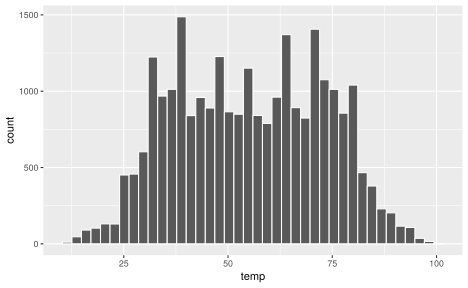
\includegraphics{lab02_rmarkdown_tutorial_files/figure-latex/unnamed-chunk-5-1.pdf}

\hypertarget{putting-an-open-street-map-under-your-map}{%
\subsection{Putting an open street map under your
map}\label{putting-an-open-street-map-under-your-map}}

Finally, it might be useful to pub a general purpose map under your map
for reference. The \texttt{annotation\_map\_tile} function in the
ggspatial package does that.

Play with the alpha level to adjust the transparancy of your thematic
map.

Also notice that I want the basemap under my choropleth, so I listed the
basemap layer before listing the geom\_sf layer. Layers are drawn in the
order in which they appear.

\begin{Shaded}
\begin{Highlighting}[]
\KeywordTok{ggplot}\NormalTok{(knox) }\OperatorTok{+}\StringTok{ }
\StringTok{  }\KeywordTok{annotation_map_tile}\NormalTok{() }\OperatorTok{+}
\StringTok{  }\KeywordTok{geom_sf}\NormalTok{(}\KeywordTok{aes}\NormalTok{(}\DataTypeTok{fill=}\NormalTok{MEDHHINC}\OperatorTok{/}\DecValTok{10000}\NormalTok{), }\DataTypeTok{alpha=}\NormalTok{.}\DecValTok{7}\NormalTok{) }\OperatorTok{+}\StringTok{ }
\StringTok{  }\KeywordTok{scale_fill_distiller}\NormalTok{(}\DataTypeTok{palette=}\StringTok{'Blues'}\NormalTok{)}\OperatorTok{+}
\StringTok{  }\KeywordTok{labs}\NormalTok{(}\DataTypeTok{fill =} \StringTok{"Median Household Income}\CharTok{\textbackslash{}n}\StringTok{($1000s)"}\NormalTok{) }\OperatorTok{+}
\StringTok{  }\KeywordTok{coord_sf}\NormalTok{(}\DataTypeTok{datum=}\OtherTok{NA}\NormalTok{)}
\end{Highlighting}
\end{Shaded}

\begin{verbatim}
## Loading required namespace: raster
\end{verbatim}

\begin{verbatim}
## Zoom: 9
\end{verbatim}

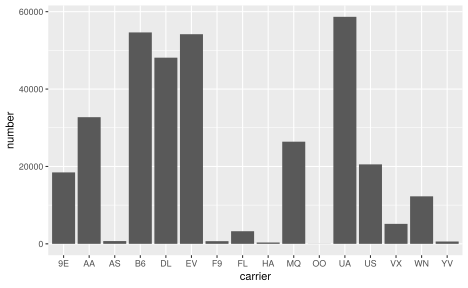
\includegraphics{lab02_rmarkdown_tutorial_files/figure-latex/unnamed-chunk-6-1.pdf}

A message saying ``zoom: 9'' is shown. It says what zoom level was
selected for the basemap. You can safely ignore it. The
annotation\_map\_tile() is pretty good at picking an appropriate zoom
level.

\hypertarget{calculating-a-correlation-coefficient-in-r.}{%
\subsection{Calculating a correlation coefficient in
R.}\label{calculating-a-correlation-coefficient-in-r.}}

The formula for correlation coefficient is \texttt{cor(x,y)}. It will
calculate the correlation coeffience between variables x and y and
return a single number. If there are missing data, it will return a
missing value to. To ignore the missing data, the function is
\texttt{cor(x,\ y,\ use\ =\ \textquotesingle{}complete.obs\textquotesingle{})}.

To calculate a correlation coefficient between Median House Value and
Median Household Income, I will show how to do that two ways: first not
using the tidyverse, and the second with the tidyverse.

\hypertarget{calculating-the-correlation-coefficient-the-non-tidyverse-way.}{%
\subsubsection{Calculating the correlation coefficient the non-tidyverse
way.}\label{calculating-the-correlation-coefficient-the-non-tidyverse-way.}}

The cor function can be used outside the tidyverse. It just needs two
columns of data. The way to access a column of data outside the
tidyverse is like so: \texttt{knox\$MEDHHINC} and
\texttt{knox\$MEDHVALUE}. The formula is
\texttt{data\_frame\$column\_name}.

\begin{Shaded}
\begin{Highlighting}[]
\NormalTok{corr_coef <-}\StringTok{ }\KeywordTok{cor}\NormalTok{(knox}\OperatorTok{$}\NormalTok{MEDHVALUE, knox}\OperatorTok{$}\NormalTok{MEDHHINC, }\DataTypeTok{use=}\StringTok{'complete.obs'}\NormalTok{)}
\NormalTok{corr_coef }\CommentTok{# Just type the object to print it out.}
\end{Highlighting}
\end{Shaded}

\begin{verbatim}
## [1] 0.8389087
\end{verbatim}

If you want to use value in a sentence, you would do it like so:
``0.8389087''. Example, the correlation coefficient betweenm Median
House Value and Median Household Income is 0.8389087.

\hypertarget{using-correlation-the-tidyverse-way}{%
\subsubsection{Using correlation the tidyverse
way}\label{using-correlation-the-tidyverse-way}}

The plan is to summarize the knox dataframe. This will create a new
dataframe. I will call the new frame summary\_stat. I will also
calculate means and standard deviations while I'm at it.

\begin{Shaded}
\begin{Highlighting}[]
\NormalTok{summary_stat <-}\StringTok{ }\NormalTok{knox }\OperatorTok
\StringTok{  }\KeywordTok{summarize}\NormalTok{(}\DataTypeTok{mean_HHINC =} \KeywordTok{mean}\NormalTok{(MEDHHINC, }\DataTypeTok{na.rm=}\OtherTok{TRUE}\NormalTok{),}
            \DataTypeTok{sd_HHINC =} \KeywordTok{sd}\NormalTok{(MEDHHINC, }\DataTypeTok{na.rm=}\OtherTok{TRUE}\NormalTok{),}
            \DataTypeTok{mean_HVALUE =} \KeywordTok{mean}\NormalTok{(MEDHVALUE, }\DataTypeTok{na.rm=}\OtherTok{TRUE}\NormalTok{),}
            \DataTypeTok{sd_HVALUE =} \KeywordTok{sd}\NormalTok{(MEDHVALUE, }\DataTypeTok{na.rm=}\OtherTok{TRUE}\NormalTok{),}
            \DataTypeTok{cor_HVALUE_HHINC =} \KeywordTok{cor}\NormalTok{(MEDHHINC, MEDHVALUE, }\DataTypeTok{use=}\StringTok{'complete.obs'}\NormalTok{))}
\NormalTok{summary_stat }\CommentTok{# just the the dataframe to print it out.}
\end{Highlighting}
\end{Shaded}

\begin{verbatim}
## Simple feature collection with 1 feature and 5 fields
## geometry type:  POLYGON
## dimension:      XY
## bbox:           xmin: -84.27347 ymin: 35.79381 xmax: -83.65092 ymax: 36.18648
## epsg (SRID):    4269
## proj4string:    +proj=longlat +datum=NAD83 +no_defs
##   mean_HHINC sd_HHINC mean_HVALUE sd_HVALUE cor_HVALUE_HHINC
## 1   56057.96 26640.32    174410.9  86960.74        0.8389087
##                         geometry
## 1 POLYGON ((-83.69458 35.9438...
\end{verbatim}

In doing that, I saw that it also printed out a bunch of stuff about the
map. We can delete that with the \texttt{df\_spatial} function in the
ggspatial package. The df\_spatial function just takes a sf object and
returns a clean (non-spatial) data frame.

\begin{Shaded}
\begin{Highlighting}[]
\NormalTok{summary_stat <-}\StringTok{ }\NormalTok{knox }\OperatorTok
\StringTok{  }\KeywordTok{df_spatial}\NormalTok{() }\OperatorTok
\StringTok{  }\KeywordTok{summarize}\NormalTok{(}\DataTypeTok{mean_HHINC =} \KeywordTok{mean}\NormalTok{(MEDHHINC, }\DataTypeTok{na.rm=}\OtherTok{TRUE}\NormalTok{),}
            \DataTypeTok{sd_HHINC =} \KeywordTok{sd}\NormalTok{(MEDHHINC, }\DataTypeTok{na.rm=}\OtherTok{TRUE}\NormalTok{),}
            \DataTypeTok{mean_HVALUE =} \KeywordTok{mean}\NormalTok{(MEDHVALUE, }\DataTypeTok{na.rm=}\OtherTok{TRUE}\NormalTok{),}
            \DataTypeTok{sd_HVALUE =} \KeywordTok{sd}\NormalTok{(MEDHVALUE, }\DataTypeTok{na.rm=}\OtherTok{TRUE}\NormalTok{),}
            \DataTypeTok{cor_HVALUE_HHINC =} \KeywordTok{cor}\NormalTok{(MEDHHINC, MEDHVALUE, }\DataTypeTok{use=}\StringTok{'complete.obs'}\NormalTok{))}
\NormalTok{summary_stat }\CommentTok{# just type the dataframe to print it out.}
\end{Highlighting}
\end{Shaded}

\begin{verbatim}
## # A tibble: 1 x 5
##   mean_HHINC sd_HHINC mean_HVALUE sd_HVALUE cor_HVALUE_HHINC
##        <dbl>    <dbl>       <dbl>     <dbl>            <dbl>
## 1     58244.   25355.     181319.    89796.            0.861
\end{verbatim}

If you want to use value in a sentence, you would do it like so:
``0.8612655''. Example, the correlation coefficient betweenm Median
House Value and Median Household Income is 0.8612655.


\end{document}
